\begin{figure}[h!]
	\centering
	
	
	
	\tikzset{every picture/.style={line width=0.75pt}} %set default line width to 0.75pt        
	
	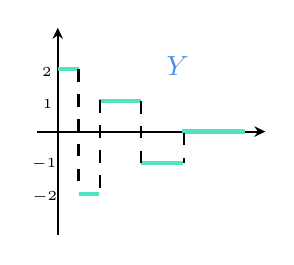
\begin{tikzpicture}[x=0.75pt,y=0.75pt,yscale=-1,xscale=1]
		%uncomment if require: \path (0,300); %set diagram left start at 0, and has height of 300
		
		%Straight Lines [id:da6563983846558457] 
		\draw    (120,130) -- (227,130) ;
		\draw [shift={(230,130)}, rotate = 180] [fill={rgb, 255:red, 0; green, 0; blue, 0 }  ][line width=0.08]  [draw opacity=0] (5.36,-2.57) -- (0,0) -- (5.36,2.57) -- (3.56,0) -- cycle    ;
		%Straight Lines [id:da6113625186161247] 
		\draw    (130,83) -- (130,180) ;
		\draw [shift={(130,80)}, rotate = 90] [fill={rgb, 255:red, 0; green, 0; blue, 0 }  ][line width=0.08]  [draw opacity=0] (5.36,-2.57) -- (0,0) -- (5.36,2.57) -- (3.56,0) -- cycle    ;
		%Straight Lines [id:da18823649577209234] 
		\draw [color={rgb, 255:red, 80; green, 227; blue, 194 }  ,draw opacity=1 ][line width=1.5]    (130,100) -- (140,100) ;
		%Straight Lines [id:da23901203978356844] 
		\draw [color={rgb, 255:red, 80; green, 227; blue, 194 }  ,draw opacity=1 ][line width=1.5]    (140,160) -- (150,160) ;
		%Straight Lines [id:da7372403791207396] 
		\draw [color={rgb, 255:red, 80; green, 227; blue, 194 }  ,draw opacity=1 ][line width=1.5]    (190,130) -- (220,130) ;
		%Straight Lines [id:da28780295701567704] 
		\draw [color={rgb, 255:red, 80; green, 227; blue, 194 }  ,draw opacity=1 ][line width=1.5]    (150,115.33) -- (170,115.33) ;
		%Straight Lines [id:da5129439211809914] 
		\draw [color={rgb, 255:red, 80; green, 227; blue, 194 }  ,draw opacity=1 ][line width=1.5]    (170.33,145) -- (190.33,145) ;
		%Straight Lines [id:da8570092074976612] 
		\draw  [dash pattern={on 4.5pt off 4.5pt}]  (140,100) -- (140,160) ;
		%Straight Lines [id:da9540488747278426] 
		\draw  [dash pattern={on 4.5pt off 4.5pt}]  (150.33,115) -- (150.33,160) ;
		%Straight Lines [id:da348777045876534] 
		\draw  [dash pattern={on 4.5pt off 4.5pt}]  (170,115.33) -- (170,146) ;
		%Straight Lines [id:da8594121119107911] 
		\draw  [dash pattern={on 4.5pt off 4.5pt}]  (190.67,130.67) -- (190.67,145) ;
		
		% Text Node
		\draw (121,97.73) node [anchor=north west][inner sep=0.75pt]  [font=\tiny]  {$2$};
		% Text Node
		\draw (116.33,157.07) node [anchor=north west][inner sep=0.75pt]  [font=\tiny]  {$-2$};
		% Text Node
		\draw (181,92.4) node [anchor=north west][inner sep=0.75pt]  [color={rgb, 255:red, 74; green, 144; blue, 226 }  ,opacity=1 ]  {$Y$};
		% Text Node
		\draw (121.33,113.07) node [anchor=north west][inner sep=0.75pt]  [font=\tiny]  {$1$};
		% Text Node
		\draw (116,141.4) node [anchor=north west][inner sep=0.75pt]  [font=\tiny]  {$-1$};
		
		
	\end{tikzpicture}
\end{figure}